\documentclass{beamer}

%------------------------------------
%------------Libraries---------------
%------------------------------------

\usepackage[portuguese]{babel}
\usepackage[utf8]{inputenc}
\usepackage[T1]{fontenc}
\usepackage{xpatch}
\usepackage{ragged2e}
\usepackage{xcolor}
\usepackage{url, hyperref}

\usepackage[percent]{overpic}

\usepackage{amsmath, amsthm, amssymb, amsfonts} 

%\usepackage{ifelse}
\usepackage{hyphenat}
\hyphenation{mate-mática recu-perar}

%------------------------------------
%----------Configurations------------
%------------------------------------

\usetheme{Madrid}
\usecolortheme{default}
\useinnertheme{circles}

\definecolor{FirstColor}{rgb}{0.0157,0.2392,0.4902}
\definecolor{SecondColor}{rgb}{0.0157, 0.549, 0.8}

\setbeamertemplate{itemize items}[triangle]

\setbeamercolor*{palette primary}{bg=FirstColor, fg=white}
\setbeamercolor*{palette secondary}{bg=SecondColor, fg=white}
\setbeamercolor*{palette tertiary}{bg=white, fg=FirstColor}
\setbeamercolor*{palette quaternary}{bg=FirstColor,fg=white}
\setbeamercolor{structure}{fg=FirstColor}
\setbeamercolor{section in toc}{fg=FirstColor}

\hypersetup{colorlinks=true,citecolor=blue, urlcolor = cien, linkcolor=blue}

\apptocmd{\frame}{}{\justifying}{}

%---------------------------------------------------
%------------------Itemize--------------------------
%---------------------------------------------------

\makeatletter
\newcommand{\my@beamer@setsep}{%
\ifnum\@itemdepth=1\relax
     \setlength\itemsep{\my@beamer@itemsepi}% separation for first level
   \else
     \ifnum\@itemdepth=2\relax
       \setlength\itemsep{\my@beamer@itemsepii}% separation for second level
     \else
       \ifnum\@itemdepth=3\relax
         \setlength\itemsep{\my@beamer@itemsepiii}% separation for third level
   \fi\fi\fi}
\newlength{\my@beamer@itemsepi}\setlength{\my@beamer@itemsepi}{3ex}
\newlength{\my@beamer@itemsepii}\setlength{\my@beamer@itemsepii}{1.5ex}
\newlength{\my@beamer@itemsepiii}\setlength{\my@beamer@itemsepiii}{1.5ex}
\newcommand\setlistsep[3]{%
    \setlength{\my@beamer@itemsepi}{#1}%
    \setlength{\my@beamer@itemsepii}{#2}%
    \setlength{\my@beamer@itemsepiii}{#3}%
}
\xpatchcmd{\itemize}
  {\def\makelabel}
  {\my@beamer@setsep\def\makelabel}
 {}
 {}

\xpatchcmd{\beamer@enum@}
  {\def\makelabel}
  {\my@beamer@setsep\def\makelabel}
 {}
 {}
\makeatother

%---------------------------------------------------
%-----------------Definitions-----------------------
%---------------------------------------------------

\newcommand{\Space}{\vspace{3ex}}

%---------------------------------------------------
%----------------Front page-------------------------
%---------------------------------------------------

\title[Respondent driven-sampling]
{Análise bayesiana de pesquisas RDS com incerteza no desfecho}
\author[Lucas Moschen]
{Lucas Moschen}
\institute[EMAp/FGV]
{
  Escola de Matemática Aplicada\\
  Fundação Getulio Vargas
}
\date[\today]
{\today}

\titlegraphic{
    \vspace*{1.2cm}
    \hspace*{9.5cm}
    
\includegraphics[width=.2\textwidth]{../rds-presentation/images/logo-emap.png}
}
%--------------------------------------------------

\AtBeginSection[]
{
  \begin{frame}
    \frametitle{Sumário}
    \tableofcontents[currentsection]
  \end{frame}
}

%---------------------------------------------------
%---------------- Document -------------------------
%---------------------------------------------------

\begin{document}

\frame{\titlepage}

%-----------------------------------------------------
\begin{frame}
\frametitle{Sumário}
\tableofcontents
\end{frame}
%----------------------------------------------------

\section{Introdução}

%---------------------------------------------------

\begin{frame}
\frametitle{Populações de difícil acesso ou ``escondidas''}

\begin{itemize}
    \justifying
    \item Não existe um esquema de amostragem clássico: tamanho e fronteiras da
    população são desconhecidos;
    \Space
    \item Preocupações com a privacidade e medo de exposição: comportamento
    estigmatizado ou ilegal;
    \Space
    \item Exemplos: Usuários de drogas pesadas, profissionais do sexo, pessoas
    em situação de rua, entre outros;
    \Space 
    \item Abordagens existentes de amostragem têm vários espaços para
    desenvolvimento.
\end{itemize}

\end{frame}

\begin{frame}
\frametitle{Respondent-driven sampling}

  \begin{itemize}
    \justifying
    \item Proposta em \cite{heckathorn1997} como uma abordagem de estimar
    proporções em uma população alvo; 

    \Space

    \item Teoria baseada em cadeias de Markov; 
    
    \Space
    
    \item \cite{crawford2016} modela como uma rede com interações e nós
    faltantes e define uma distribuição de probabilidade sobre o subgrafo
    observado;
    
    \Space 

    \item Amostragem sem reposição. 

  \end{itemize}

\end{frame}

\begin{frame}{Estudo RDS: refugiados e ativistas na Síria}
  \begin{figure}
    \begin{overprint}
    \onslide<1>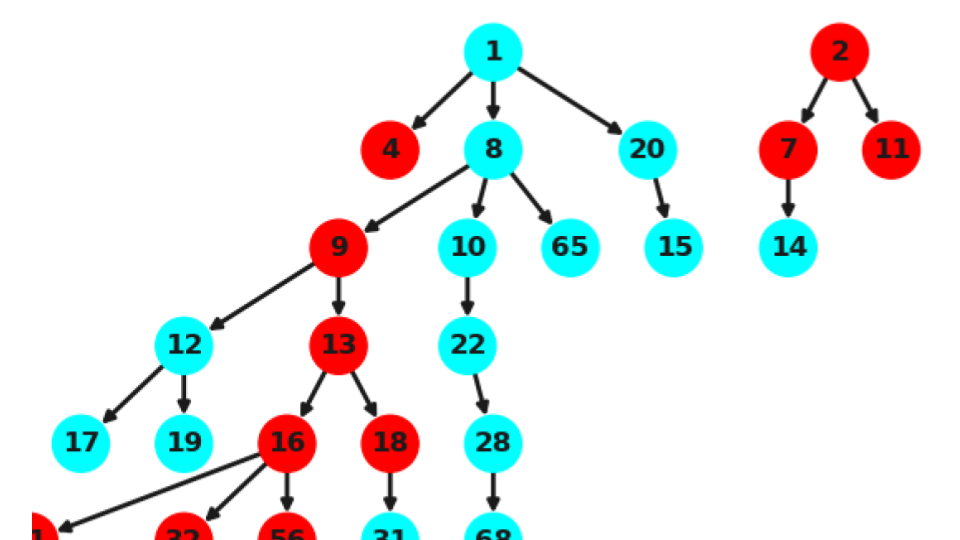
\includegraphics[width=\textwidth]{../../images/graph-rds-harvard-1.png}
    \onslide<2>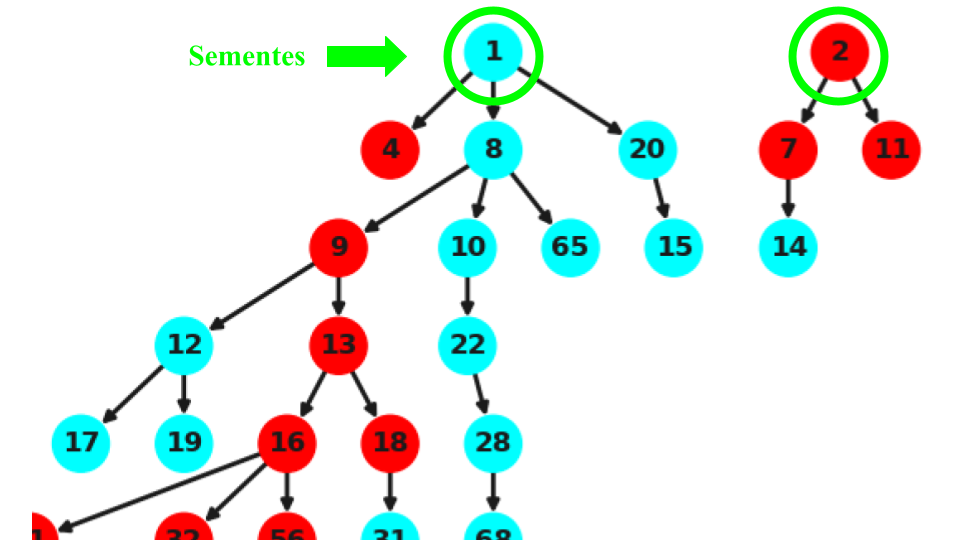
\includegraphics[width=\textwidth]{../../images/graph-rds-harvard-2.png}
    \onslide<3>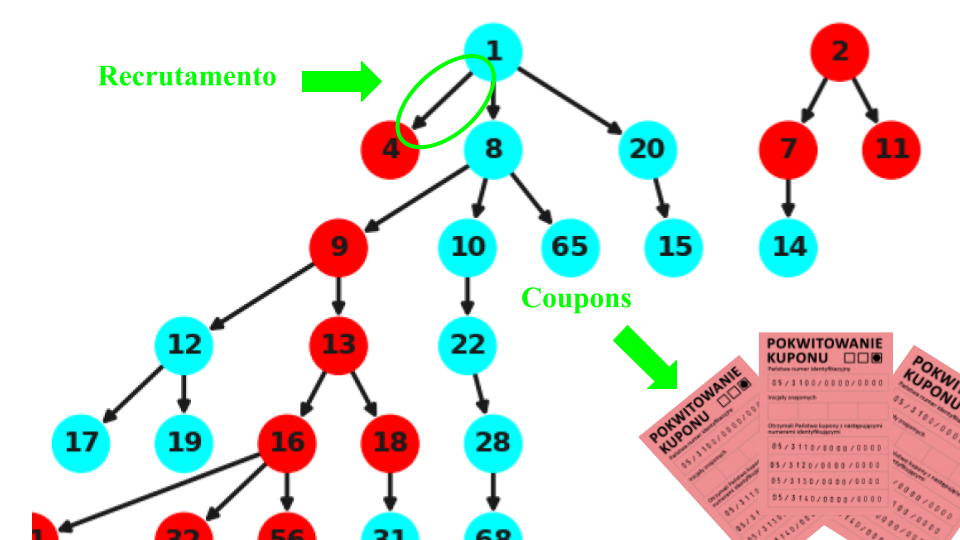
\includegraphics[width=\textwidth]{../../images/graph-rds-harvard-3.png}
    \onslide<4>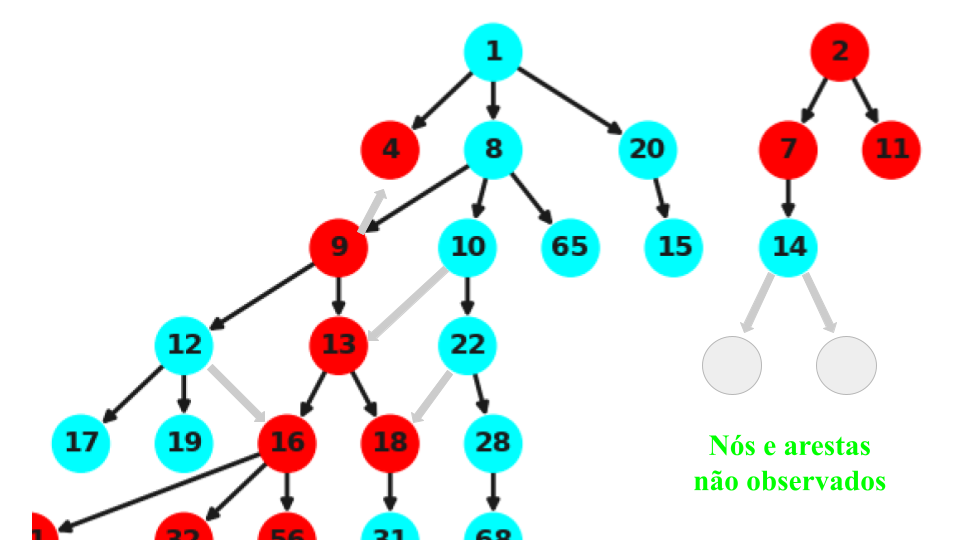
\includegraphics[width=\textwidth]{../../images/graph-rds-harvard-4.png}
    \end{overprint}
  \end{figure}  
\end{frame}

\begin{frame}{Estimação de prevalência com testes imperfeitos}
  \begin{figure}
    \begin{overprint}
    \onslide<1>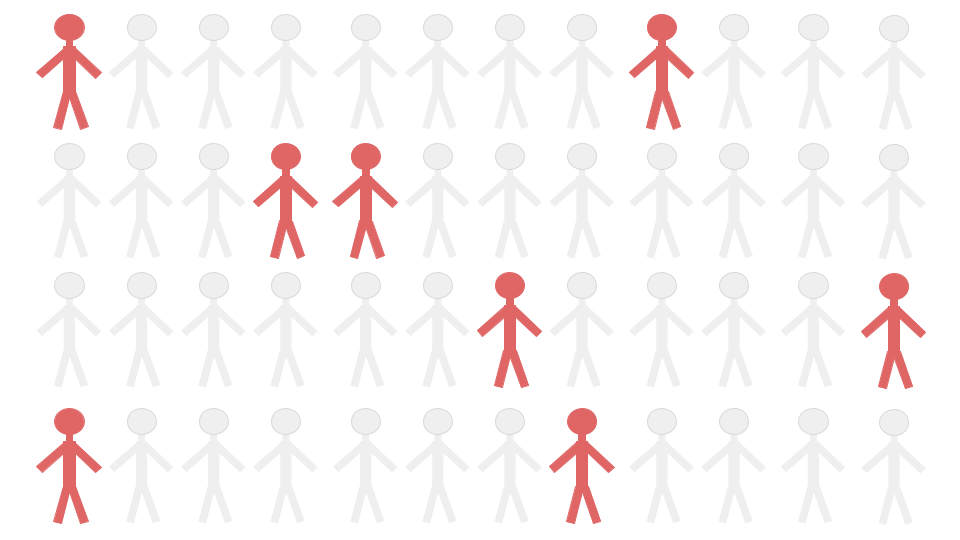
\includegraphics[width=\textwidth]{../../images/prevalence-1.png}
    \onslide<2>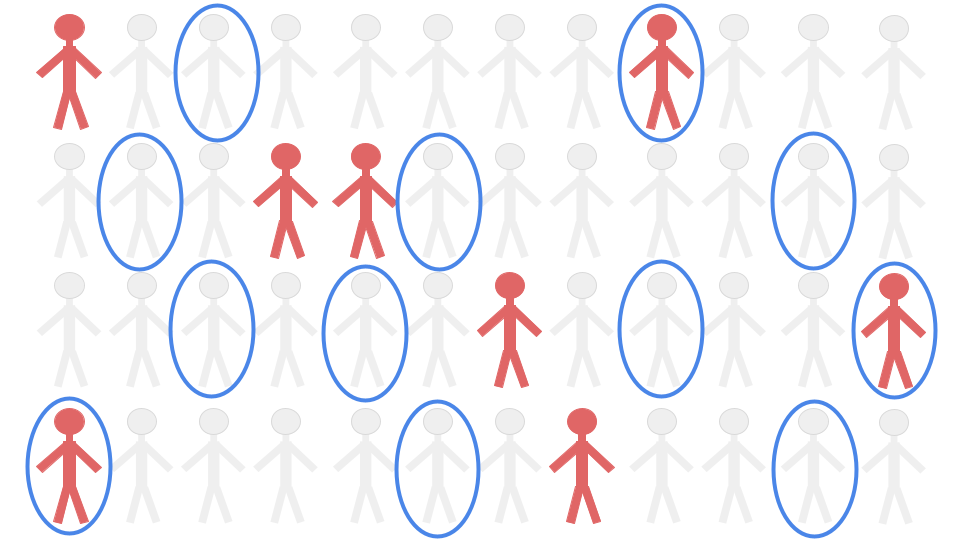
\includegraphics[width=\textwidth]{../../images/prevalence-2.png}
    \onslide<3>\begin{overpic}[width=\textwidth]{../../images/prevalence-3.png}
    \put (62.5,33) {A média da amostra,} 
    \put (57.2,28) {{\em prevalência aparente} e {\em MLE},} 
    \put (60.5,23) {é um possível estimador.}
     \end{overpic}
    \end{overprint}
  \end{figure}  
\end{frame}

\begin{frame}{Especificidade e Sensibilidade}

  {\bf Especificidade:} Probabilidade de resultado negativo nos não doentes.

  \vspace{2mm}
  {\bf Sensibilidade:} Probabilidade de resultado positivo nos doentes.
  \begin{figure}
    \centering
    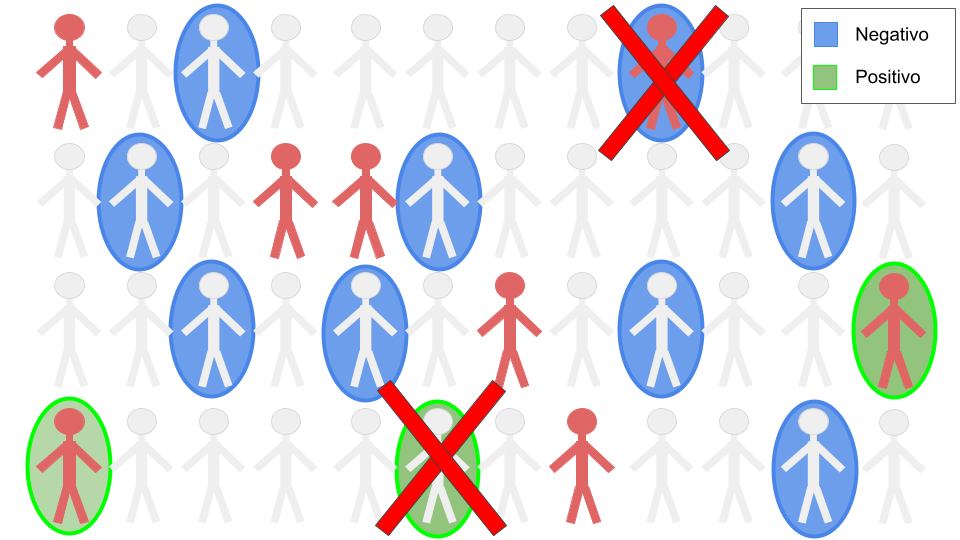
\includegraphics[width=0.95\textwidth]{../../images/prevalence-4.png}
  \end{figure}
\end{frame}

\begin{frame}{Estatística bayesiana}

  \begin{itemize}
    \item Interpretação baseada no grau de crença em uma afirmação por um
    indivíduo;

    \Space

    \item A fórmula de Bayes relaciona a probabilidade de um parâmetro após
    observar novos dados com a evidência e a informação prévia sobre ele;

    \Space

    \item Permite a quantificação da incerteza de uma forma direta, dado que o
    processo não precisa ser aleatório.
  \end{itemize}

\end{frame}

%----------------------------------------------------

\section{Justificativa}

\begin{frame}{Justificativa}
  \begin{itemize}

    \justifying

    \item Populações escondidas são sub-representadas em pesquisas nacionais e
    têm maior risco de abuso de drogas ou contrair infecções sexualmente
    transmissíveis;

    \Space
    
    \item O tópico tem vários gaps na estatística e abordagens de regressão
    para estimar prevalência considerando a estrutura de rede podem ser
    construídas \cite{bastos2012binary}.
  \end{itemize}
\end{frame}

%---------------------------------------------------

%----------------------------------------------------

\section{Objetivos}

\begin{frame}{Objetivo geral}

  \justifying

  Este trabalho tem o objetivo de estudar o problema da estimação de
  prevalência em uma estrutura de rede RDS considerando a Especificidade e a
  Sensitividade do diagnóstico. 

  \Space
  
  Também se pretende aplicar esse framework de
  forma eficiente, comparando algoritmos Monte Carlo e Aproximações de Laplace. 
\end{frame}

\begin{frame}{Específicos}

  \begin{enumerate}

    \justifying

    \item Revisão bibliográfica, descrição matemática do problema e propagação
    da incerteza com métodos Bayesianos; 

    \Space

    \item Distribuição conjunta a priori da especificidade e sensibilidade;
    
    \Space

    \item Implementação eficiente utilizando pacotes estatísticos, como {\em rstanarm} e {\em INLA};
    
    \Space

    \item Análise de estudos epidemiológicos RDS.
  \end{enumerate}
  
\end{frame}

%---------------------------------------------------

%----------------------------------------------------

\section{Metodologia}

%---------------------------------------------------

\begin{frame}{Metodologia}

{\bf Pesquisa bibliográfica}

A fundamentação teórica se dará por meio de artigos nos tópicos indicados na
introdução: RDS, estimativa de prevalência por meio de
regressão, e estatística bayesiana. 

\Space

{\bf Recursos técnicos}

Toda a programação necessária será feita nas linguagens de programação \textit{Python} e \textit{R}. 

\Space

{\bf Estudo formal}

Disciplinas do Doutorado em Modelagem Matemática da EMAp: Estatística Bayesiana e Ciências de Redes.

\end{frame}

%----------------------------------------------------

\section{Resultados preliminares}

%---------------------------------------------------

\begin{frame}
  
  Observe also that for a network the independence of the sample is
  also not valid. Other estimators are better. Adicionar o modelo 1 e comentar
  sobre a beta bivariada.
  
  Se $\pi$ é a probabilidade do teste ser positivo,
  $$
  \pi = \theta\gamma_s + (1-\theta)(1-\gamma_e),
  $$
  e podemos estudar $\theta$ considerando $\gamma_s, \gamma_e$. 

\end{frame}

%----------------------------------------------------

\section{Cronograma}

\begin{frame}{Cronograma}
  
\end{frame}

%---------------------------------------------------

\begin{frame}[t, allowframebreaks]
   \frametitle{References}
   \bibliographystyle{apalike}
   \bibliography{../tcc-project/biblio}
 \end{frame}

\end{document}